\section{Evaluation}
% Met een subsectie voor elke deelvraag.
% In hoeverre is je vraag beantwoord?
% Een mooie graphic/visualisatie is hier heel gewenst.
% Hou het kort maar krachtig.

\subsection{RQ1}
\textbf{Which way of pooling vectors to a fixed length works best for classifying fake news?}\\
The answer to this question will be given by comparing accuracy of a logistic regression with different pooling strategies (max, min, average).

\begin{figure}[h]
    \centering
    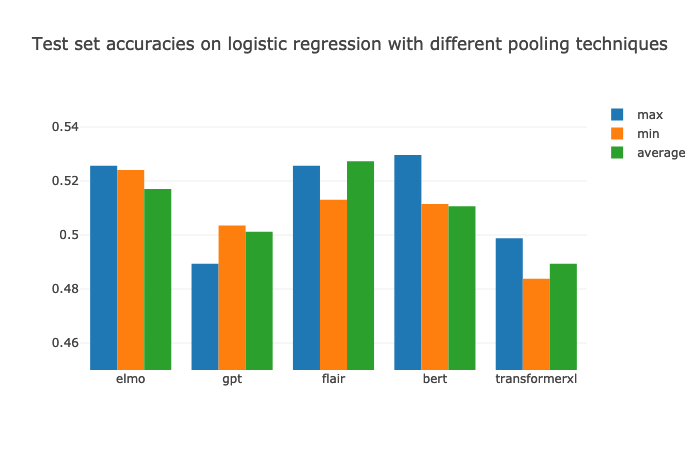
\includegraphics[scale=0.4]{poolingaccuracy}
    \caption{Comparing different pooling strategies.}
\end{figure}

\subsection{RQ2}
\textbf{At what padding sequence length do neural networks hold the highest accuracy when classifying fake news?}\\
The answer to this question will be given by comparing accuracy of a bidirectional LSTM architecture with variable padding lengths.

\begin{figure}[h]
    \centering
    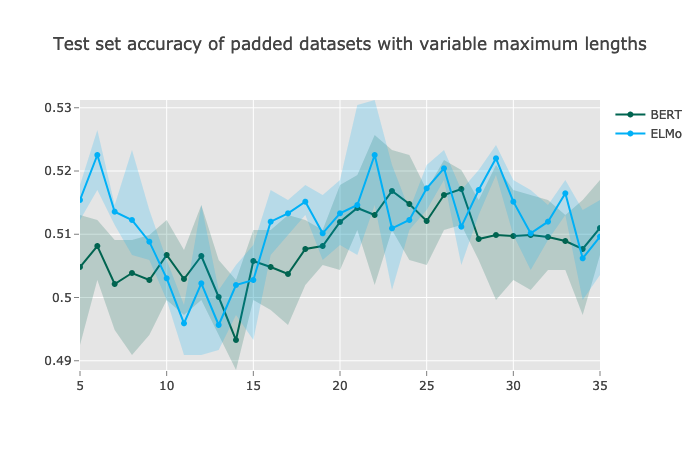
\includegraphics[scale=0.4]{padaccuracy}
    \caption{Comparing different maximum padding lengths.}
\end{figure}

By comparing all embedding techniques, I plan on getting a peak padding length with the best overall performance shared by all embedding methods. 
At this moment, the optimal length averages at around a length of 22. 

\subsection{RQ3}
\textbf{How well do neural network classification architectures classify fake news compared to non-neural classification algorithms?}\\
The answer of this question will be given by comparing two linear classifiers with two neural classifiers. 

\begin{figure}[h]
    \centering
    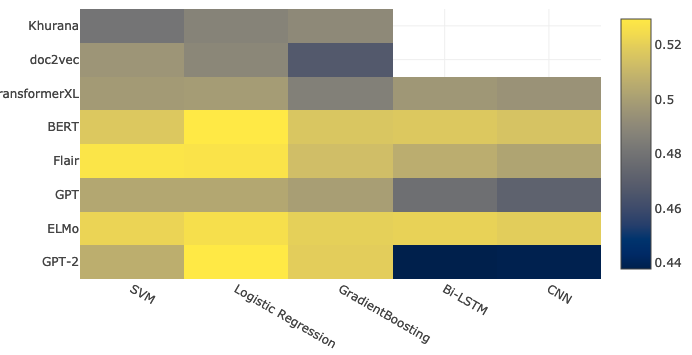
\includegraphics[scale=0.4]{linearvsneural}
    \caption{Comparing linear classifiers with neural classifiers.}
\end{figure}

\pagebreak